% Section content template for individual Educative lessons
% This file contains the actual content for a specific section
% Generated from Educative API section content

% Section: Quiz: Object-Oriented Design Principles
% Section ID: 4522841418760192
% Section Slug: quiz-object-oriented-design-principles
% Generated: 2025-12-11T05:50:47.580109

\subsection{MCQs}\label{MCQs}
\\
Challenge yourself by solving the following quiz questions.

\subsection*{Quiz: Object-Oriented Design Principles}
\vspace{0.3cm}
\noindent
\textbf{Question 1:} What best demonstrates a violation of the Single Responsibility principle (SRP)?
\\[0.2cm]
\begin{itemize}
 \item A class that only handles user authentication
 \item \textbf{[CORRECT]} A class that manages user login, prints invoices, and saves data to a database
\\[0.1cm]
\textit{Explanation:} 
The class in option B is taking on multiple unrelated responsibilities---managing login, printing invoices, and saving to a database---violating SRP, which states a class should have only one reason to change.
 \item A class that calculates the total price of items in a cart
 \item A class that represents a book with title and author as properties
\end{itemize}
\vspace{0.3cm}
\noindent
\textbf{Question 2:} Given a class that prints an invoice and saves it to the database, how should it be refactored to follow the Single Responsibility principle?
\\[0.2cm]
\begin{itemize}
 \item \textbf{[CORRECT]} Move printing and saving methods to separate classes.
\\[0.1cm]
\textit{Explanation:} 
To follow SRP, each responsibility (printing and saving) should be moved to its own class (e.g., InvoicePrinter and InvoiceStorage), so each class has only one reason to change.
 \item Add more methods to handle different formats.
 \item Combine all methods in a utility class.
 \item Only keep the saving method and remove printing functionality.
\end{itemize}
\vspace{0.3cm}
\noindent
\textbf{Question 3:} \textbf{(True or False)}
\\
The Open/Closed principle states that software entities should be open for modification but closed for extension.
\\[0.2cm]
\begin{itemize}
 \item True
 \item \textbf{[CORRECT]} False
\\[0.1cm]
\textit{Explanation:} 
The principle states that entities should be open for extension but closed for modification. You should be able to add new functionality without modifying existing code.
\end{itemize}
\vspace{0.3cm}
\noindent
\textbf{Question 4:} A developer must add support for a new box shape to an existing volume calculation system without changing the core calculation logic.
\\
Which SOLID principle is most relevant here, and what should the developer do?
\\[0.2cm]
\begin{itemize}
 \item SRP: Add the logic to the main class.
 \item \textbf{[CORRECT]} OCP: Create a new shape subclass and override the volume method.
\\[0.1cm]
\textit{Explanation:} 
According to OCP, the system should be extendable (by creating a new shape subclass) without modifying existing code.
 \item LSP: Change all classes to inherit from a base class.
 \item DIP: Make all classes depend on concrete classes.
\end{itemize}
\vspace{0.3cm}
\noindent
\textbf{Question 5:} What is a sign that the Liskov Substitution principle (LSP) has been violated?
\\[0.2cm]
\begin{itemize}
 \item A subclass adds new optional methods.
 \item \textbf{[CORRECT]} A subclass throws an error when a superclass method is called.
\\[0.1cm]
\textit{Explanation:} 
If a subclass cannot properly implement or support a method from its superclass and throws errors when that method is called, it violates LSP.
 \item A subclass overrides a method with improved performance.
 \item A subclass adds extra properties.
\end{itemize}
\vspace{0.3cm}
\noindent
\textbf{Question 6:} In a vehicle system, adding a \texttt{startEngine()} method to the \texttt{Vehicle} base class causes a problem when a \texttt{Bicycle} subclass is added. What is the best way to resolve this violation of LSP?
\\[0.2cm]
\begin{itemize}
 \item Remove the \texttt{Bicycle} class.
 \item \textbf{[CORRECT]} Move \texttt{startEngine} to a \texttt{MotorizedVehicle} subclass and have \texttt{Bicycle} inherit from a different base.
\\[0.1cm]
\textit{Explanation:} 
By creating separate hierarchies for \texttt{MotorizedVehicle} and \texttt{ManualVehicle}, you allow classes to only implement what makes sense for them, respecting LSP.
 \item Make all vehicles have dummy \texttt{startEngine} methods.
 \item Remove inheritance altogether.
\end{itemize}
\vspace{0.3cm}
\noindent
\textbf{Question 7:} Assume we have a \texttt{Student} class that contains the database of all the students present in a school.
\\
The \texttt{Student} class has two main functionalities as follows:

\begin{itemize}
\tightlist
\item
Add any new students to the school database.
\item
Access and display the details of any existing students.
\end{itemize}
\\
How should the \texttt{Student} class be updated to apply the Interface Segregation principle?
\\[0.2cm]
\begin{itemize}
 \item The \texttt{Student} class itself should contain two methods for adding students and accessing students.
 \item \textbf{[CORRECT]} The \texttt{Student} class should be divided into two separate classes for adding students and accessing students.
 \item The \texttt{Student} class should only contain the \texttt{addingStudents} method. There should be a separate class for accessing students' functionality.
 \item The \texttt{Student} class should only contain the \texttt{accessingStudents} method. There should be a separate class for adding students' functionality.
\end{itemize}
\vspace{0.3cm}
\noindent
\textbf{Question 8:} \textbf{(True or False)} The Interface Segregation principle recommends having large, general-purpose interfaces so classes can implement as many features as possible.
\\[0.2cm]
\begin{itemize}
 \item True
 \item \textbf{[CORRECT]} False
\\[0.1cm]
\textit{Explanation:} 
ISP recommends small, specific interfaces to avoid forcing classes to implement methods they don't need.
\end{itemize}
\vspace{0.3cm}
\noindent
\textbf{Question 9:} An abstract class, \texttt{Vehicle}, inherits the classes \texttt{Bicycle} and \texttt{Carriage} as its subclasses. The
\texttt{Vehicle} class contains a pure virtual function, \texttt{startMoving(),} and is implemented in both subclasses. Suppose we need another vehicle type, such as \texttt{Car}, in a system with an \texttt{addFuel()} function. Let
's also suppose we decide to inherit the \texttt{Car} class from the \texttt{Vehicle} class and fulfill the \texttt{addFuel()} functionality as shown in the figure:
\\
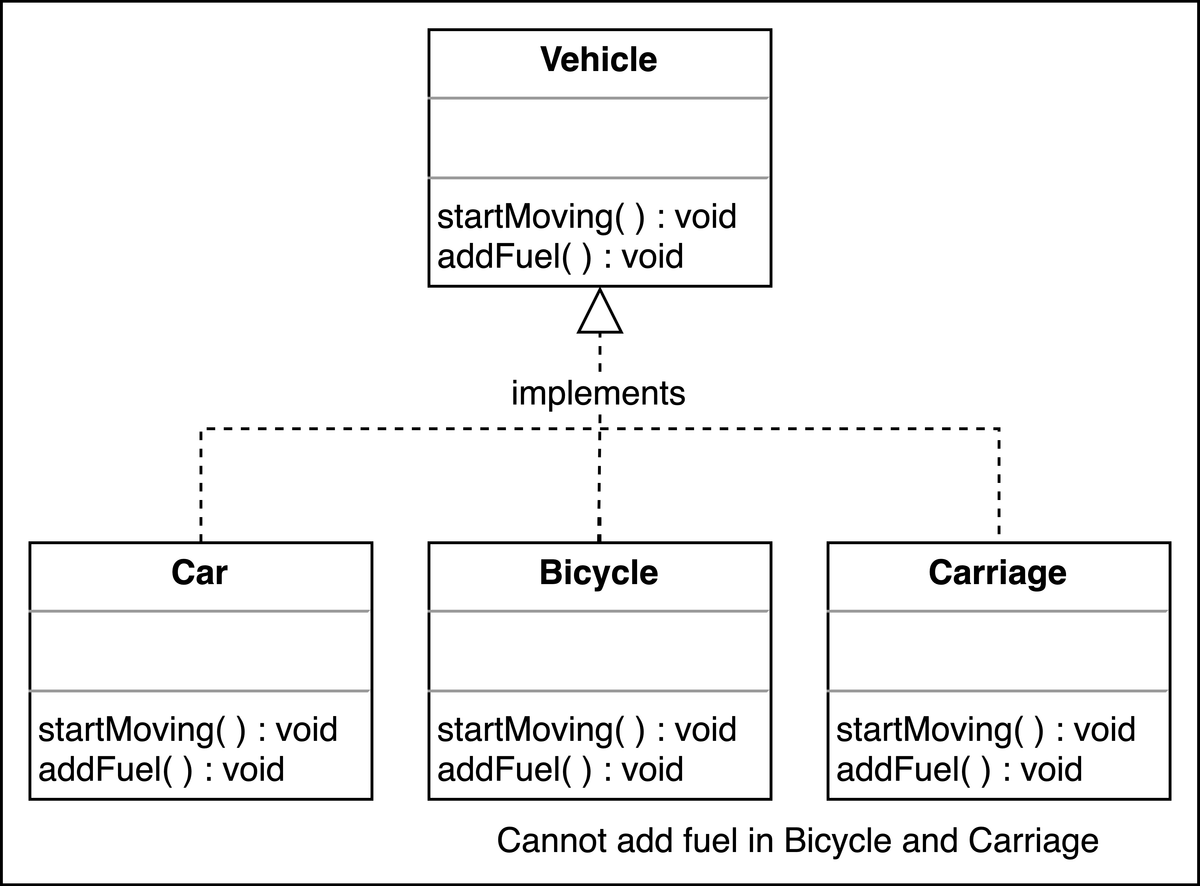
\includegraphics[width=3.64583in,height=\textheight,keepaspectratio]{Images/chapter_4/udata/Q8.png}
\\
Which design principle is violated by this implementation?
\\[0.2cm]
\begin{itemize}
 \item Single Responsibility principle
 \item Open/Closed principle
 \item Liskov Substitution principle
 \item \textbf{[CORRECT]} Interface Segregation principle
\end{itemize}
\vspace{0.3cm}
\noindent
\textbf{Question 10:} An abstract class, \texttt{Vehicle,} inherits the classes \texttt{Bicycle} and \texttt{Carriage} as its subclasses. The
\texttt{Vehicle} class contains a pure virtual function, \texttt{startMoving(),} which is implemented in both subclasses. Suppose we need another vehicle type, such as \texttt{Car,} in a system that also has an \texttt{addFuel()} function.
\\
What is the correct implementation of the above scenario?
\\[0.2cm]
\begin{itemize}
 \item 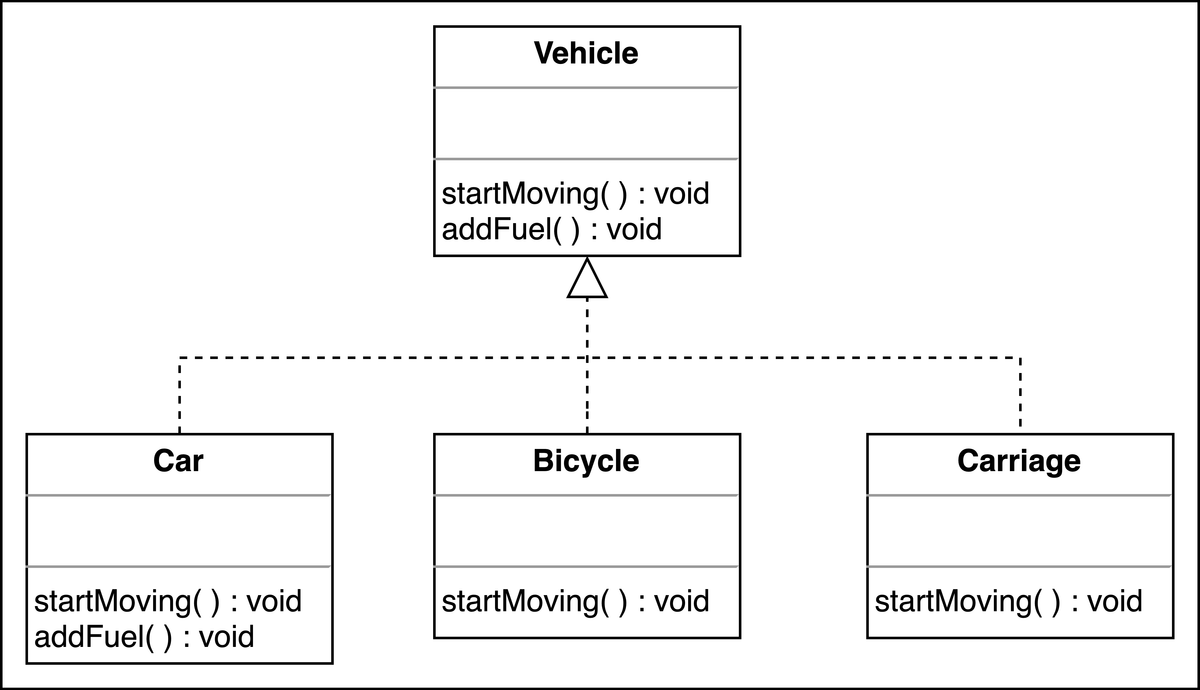
\includegraphics[width=3.125in,height=\textheight,keepaspectratio]{Images/chapter_4/udata/1.png}
 \item 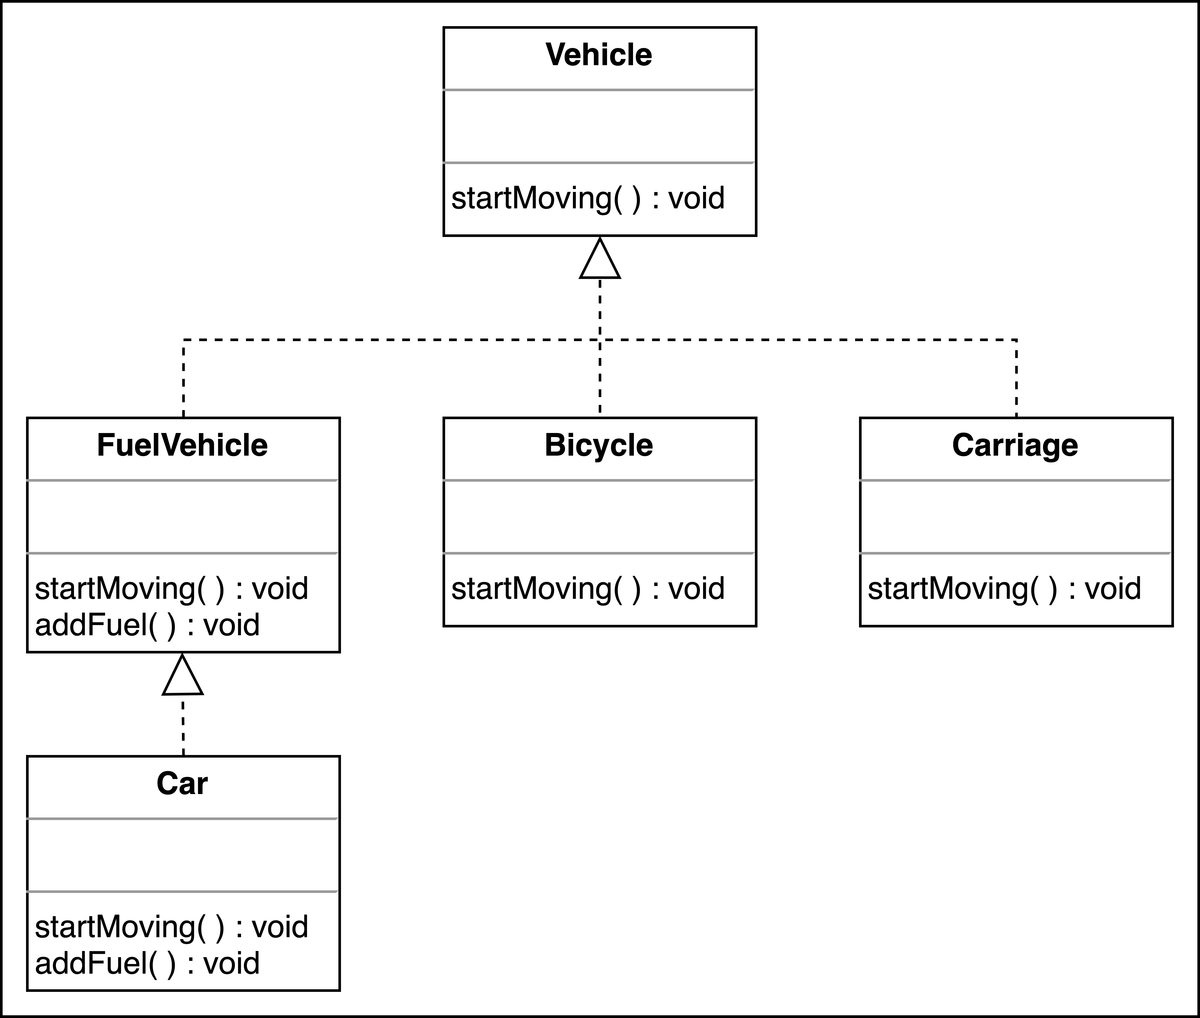
\includegraphics[width=3.125in,height=\textheight,keepaspectratio]{Images/chapter_4/udata/q9b.png}
 \item 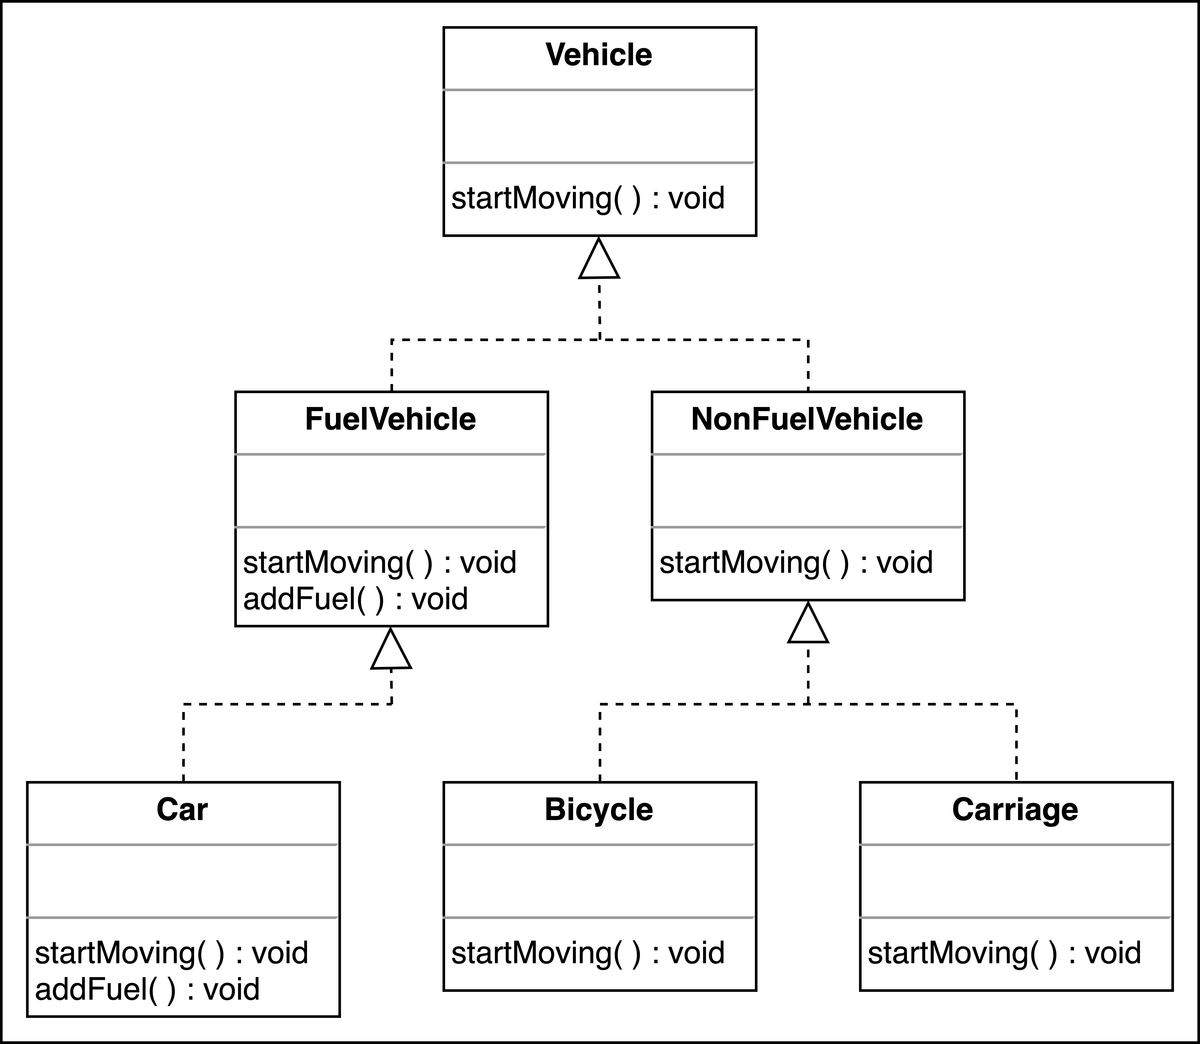
\includegraphics[width=3.125in,height=\textheight,keepaspectratio]{Images/chapter_4/udata/q9c.png}
 \item \textbf{[CORRECT]} Both B and C
\end{itemize}



% End of section content